Retinal ganglion cells (RGCs) are the only retinal neurons that send axons out of the eyes.
RGC axons navigate to the optic disc at the back of the retina and then out of the eye into the optic nerve.
After extending along the length of the optic nerve, RGC axons next navigate the optic chiasm, the midline choice point of the visual system.
In primates, whose eyes are located more frontally on the head, roughly half of the RGC axons cross the midline through the optic chiasm, and the other half project ipsilaterally after being repelled away from the chiasm.
This choice at the optic chiasm is what underlies binocular vision - each hemisphere of the brain receives input from both eyes.
In animals with more laterally positioned eyes, and therefore less binocular vision, more RGC axons project contralaterally at the optic chiasm.
In mice, which have relatively poor binocular vision, roughly 3-5\% of RGCs project ipsilaterally at the midline, leaving the vast majority to cross the midline and project contralaterally \cite{petros2008retinal}.

\begin{figure}[hbtp]
	\begin{center}
		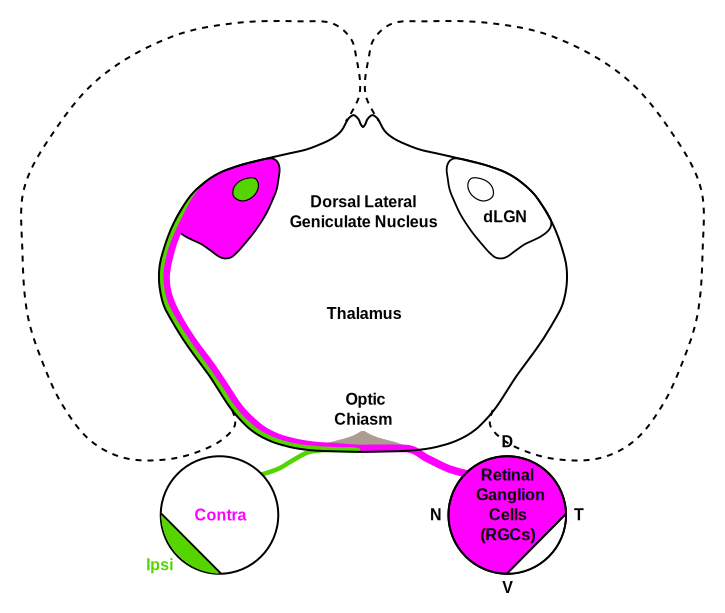
\includegraphics[width=\textwidth]{Figures/RGP_Schema.svg}
		\caption{The mouse retinogeniculate system. Contralateral RGC axons (magenta) cross at the optic chiasm and ipsilateral RGC axons (green), which arise in the ventrotemporal (VT) retina only, turn away from the chiasm. The cortex is shown with dashed lines for context. The schematic is shown in a frontal view.}
		\label{Figures/RGP_Schema}
	\end{center}
\end{figure}
After navigating the optic chiasm, ipsilateral (ipsi) and contralateral (contra) RGC axons run in the optic tract and project into the dorsal lateral geniculate nucleus (dLGN), and further dorsally and caudally, into the superior colliculus (SC).
Relay neurons in the dLGN and SC then project to the visual cortex for higher order visual processing.
For the purposes of my thesis, I have focused only on the projections of RGC axons to the dLGN, as this includes the majority of the optic tract.
The retinogeniculate pathway is schematized in Figure~\ref{figures/RGP_Schema}, with ipsi RGC axons colored in green and contra in magenta.
This color scheme will be used throughout the thesis for consistency.

\begin{figure}[hbtp]
	\begin{center}
		\includegraphics[width=\textwidth]{Figures/RGP_DevSeries.svg}
		\caption{Three phases of axon outgrowth from the mouse retina. In the early phase of RGC axon outgrowth, at left, both ipsi and contra RGCs arise in the central retina. RGC differentiation continues in a center-to-periphery wave. During the peak phase of axon outgrowth, ventrotemporal (VT) retina produces predominantly ipsi RGCs, with contras arising everywhere else. Finally, at right, during the late phase of axon outgrowth, the VT retina produces both ipsi and contra RGCs.}
		\label{Figures/RGP_DevSeries}
	\end{center}
\end{figure}
While eye-specific zones in primates and carnivorous mammals are organized into laminae, the mouse dLGN has a center-surround organization of ipsi and contra zones.
These eye-specific zones are refined from coarsely targeted axon terminals in the first two weeks of postnatal life, largely by activity-dependent refinement \cite{huberman2008mechanisms,feldheim2010visual}.
As shown in Figure~\ref{Figures/RGP_DevSeries}, RGC axon outgrowth from the retina occurs in three phases during embryogenesis.
In the early phase, from embryonic day (E) 11 or 12 to E14, the central retina produces both ipsi and contra RGCs.
This population of early-born ipsi RGCs is transient, and does not contribute to the permanent ipsi population arising from the VT retina later \cite{drager1985birth,colello1990early,soares2015transient}.
E14-16 marks the peak phase of RGC axon outgrowth from the retina, when the VT retina prodcues predominantly ipsi RGCs \cite{drager1985birth,petros2008retinal}.
While it is apparent that VT retina is predominantly ipsi during this period, the extent of heterogeneity in the VT retina is still unclear and details are currently being more closely examined {Marcucci \& Mason, unpublished}.
In the late phase of axon outgrowth, from E17 to birth, VT retina produces both ipsi and contra RGCs \cite{drager1985birth,petros2008retinal}.
These late-born VT contra RGCs target the dorsal tip of the dLGN (not shown in Figure~\ref{Figures/RGP_DevSeries}), in a markedly different position than their VT ipsi RGC counterparts, which all cluster in the central zone of the dLGN.